\section{Dynamic Programming}

% https://www.sciencedirect.com/topics/computer-science/dynamic-programming

Dynamic programming is an optimization method based on the principle of optimality 
defined by Bellman in the 1950s: “An optimal policy has the property that whatever 
the initial state and initial decision are, the remaining decisions must constitute 
an optimal policy with regard to the state resulting from the first decision.”

It can be summarized simply as follows: {\bf \textcolor{magenta}{“every optimal policy consists only of 
optimal sub policies.”}}

This method is a variant of the “divide and conquer” method given that a solution 
to a problem depends on the previous solutions obtained from subproblems. The main 
and major difference between these two methods relates to the superimposition of 
subproblems in dynamic programming. A subproblem can be used to solve a number of 
different subproblems. In the “divide and conquer” approach, subproblems are 
entirely independent and can be solved separately. Moreover, recursion is used, 
unlike in dynamic programming where a combination of small subproblems is used to 
obtain increasingly larger subproblems.

To sum up, it can be said that the “divide and conquer” method works by following 
a top-down approach whereas dynamic programming follows a bottom-up approach.

How these two methods function can be illustrated and compared in two arborescent graphs.

\begin{figure}[!htb]
\centering
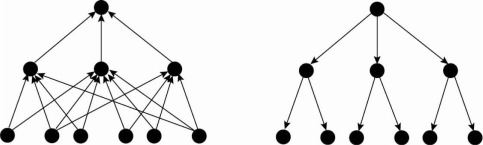
\includegraphics[scale=0.8]{pix/dnc_dp.jpg}
\caption{The methods: dynamic programming (left) and divide and conquer (right)}
%\label{fig:label}
\end{figure}




\subsection{Bellman backup equation}


\begin{tikzpicture}[->,>=stealth',level/.style={sibling distance = 5cm/#1,
  level distance = 1.5cm}] 
\node [arn_n] {33}
    child{ node [arn_r] (test0) {15}
        {
            child{ node [arn_n] {10}
                {
                % edge from parent node[above left] {$r$}
                edge from parent node[below left] (A) { \makebox[8em][l]{$q_\pi(s',a') \leftarrowtail a'$} }
                }
            }
            child{ node [arn_n] {20} }
            edge from parent node[below left] (A) { \makebox[4em][l]{$s'$} }
        } edge from parent node[left] {$r$} %for a named pointer
    }
    child{ node [arn_r] (test1) {47}
            child{ node [arn_n] {38} }
            child{ node [arn_n] {51} }
	}edge from parent node[left] (A) {\makebox[7em][l]{$q_\pi(s,a) \leftarrowtail s, a$}}
    
    ;

    %\filldraw[red] (A) circle[radius=1pt];
\end{tikzpicture}

Bellman Equations are recursive relationships among values that can be used 
to compute values.

\begin{equation}\label{bellman_equation_DP}
q_\pi(s,a) = r(s,a) + \gamma \sum_{s'\in \mathcal{S}}\mathcal{P}_{ss'}^a 
\sum_{a'\in \mathcal{A}} \pi(a'|s')q_n(s',a')
\end{equation}


% file:///D:/mygit/ml/reinforcementLearning/refs/bellman/6%20Bellman%20Eqs%20and%20DP.pdf

\begin{figure}[!htb]
\centering
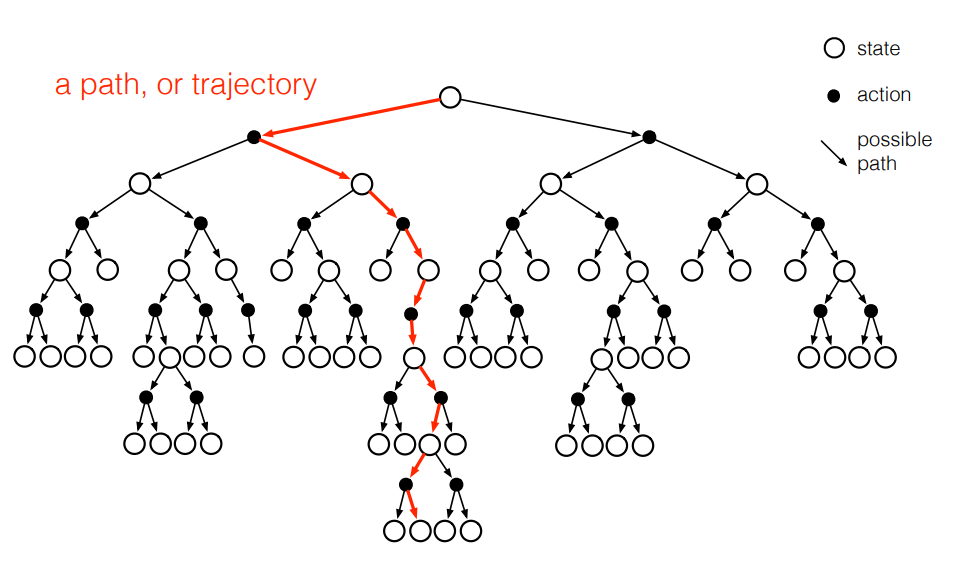
\includegraphics[scale=0.7]{pix/tee-transition-dynamics.png}
\caption{The tree of transition dynamics}
%\label{fig:label}
\end{figure}


\begin{figure}[!htb]
\centering
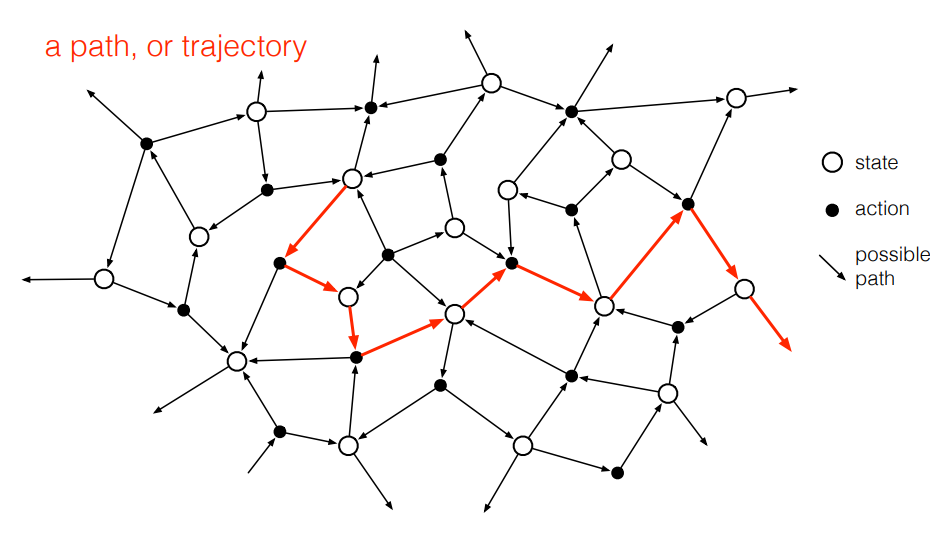
\includegraphics[scale=0.7]{pix/web-transition-dynamics.png}
\caption{The web of transition dynamics}
%\label{fig:label}
\end{figure}


\begin{figure}[!htb]
\centering
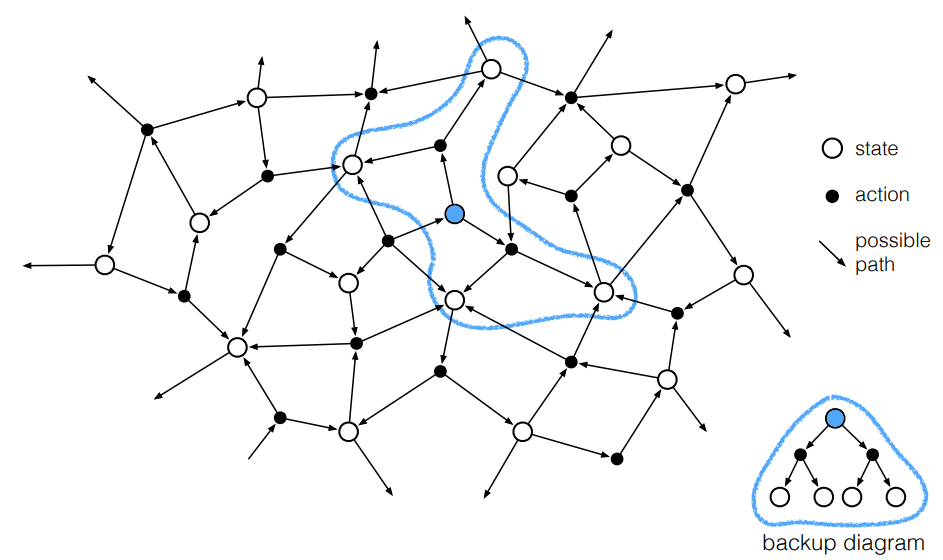
\includegraphics[scale=0.7]{pix/web2-transition-dynamics.png}
\caption{The web of transition dynamics}
%\label{fig:label}
\end{figure}


\subsection{4 Bellman-equation backup diagrams}

\begin{figure}[!htb]
\centering
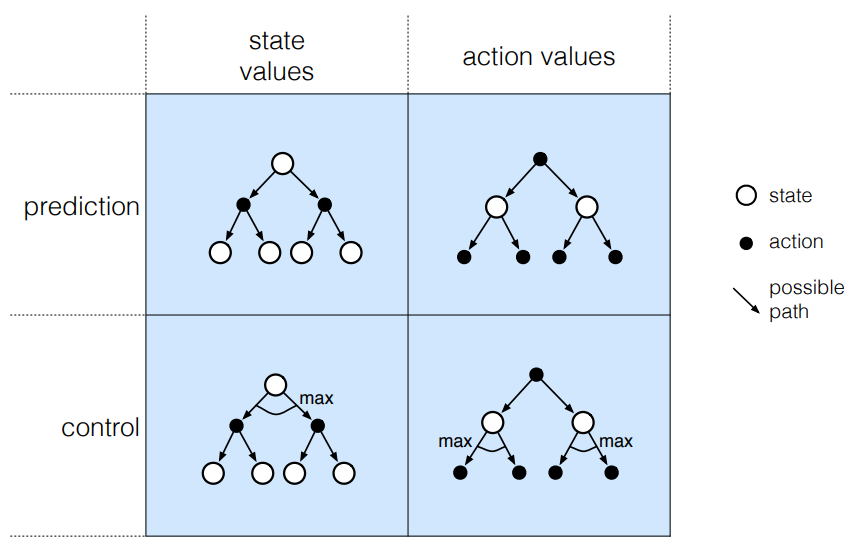
\includegraphics[scale=0.7]{pix/4-backup-diagrams.png}
\caption{4 Bellman-equation backup diagrams}
%\label{fig:label}
\end{figure}


\subsection{Bellman Equation for a Policy $\pi$}

这里的内容可对照 mdp 相应的部分。The return $G_t$ is the total discounted reward from $t$.
The discount rate $\gamma$ determines the present value of future rewards: a 
reward received $k$ time steps in the future is worth only $\gamma^{k-1}$ times 
what it would be worth if it were received immediately. And also, it provides 
mathematical convenience since as $k\rightarrow\infty$ then $\gamma^k\rightarrow 0$.

The basic idea:

\begin{align*}
G_t &= R_{t+1} + \gamma R_{t+2} + \gamma^2 R_{t+3} + \gamma^3 R_{t+4} + \cdots \\
&= R_{t+1} + \gamma \left( R_{t+2} + \gamma R_{t+3} + \gamma^2 R_{t+4} + \cdots \right) \\
&= R_{t+1} + \gamma G_{t+1}
\end{align}

So:
\begin{emp_box}
\begin{align*}
v_\pi(s) &= \mathbb{E}_\pi\left\{ G_t | S_t = s \right\} \\
&= \mathbb{E}_\pi\left\{ R_{t+1} + \gamma v_\pi\left( S_{t+1} \right) | S_t = s \right\}
\end{align}
\end{emp_box}

Or, without the expectation operator:
$$
v_\pi(s) = \sum_a \pi(a|s) \sum_{s',r} p(s', r | s, a) \left[ r + \gamma v_\pi(s') \right]
$$
This is a set of equations (in fact, linear), one for each state. The value function 
for $\pi$ is its unique solution.


\begin{figure}[!htb]
\centering
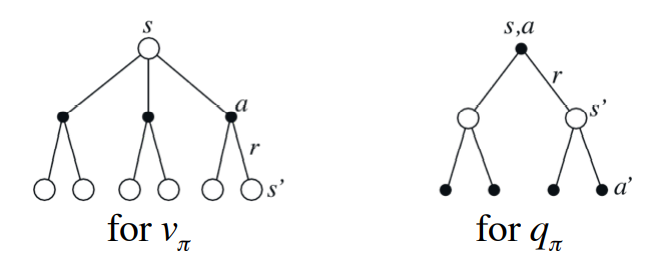
\includegraphics[scale=0.7]{pix/backup_diagrams.png}
\caption{Backup diagrams}
%\label{fig:label}
\end{figure}


\subsection{Policy Evaluation}
% http://www.incompleteideas.net/book/ebook/node41.html

First we consider how to compute the state-value function $V^*$ for an arbitrary 
policy $\pi$. This is called {\bf policy evaluation} in the DP literature. We also 
refer to it as the {\bf prediction problem}. Recall in RL that, for all $s \in \mathcal{S}$,

\begin{align}
V^\pi(s) &= \mathbb{E}_\pi\left\{ 
r_{t+1} + \gamma r_{t+2} + \gamma^2 r_{t+3} + \gamma^3 r_{t+4} + \cdots | s_t = t 
\right\} \notag \\
&= \mathbb{E}_\pi\left\{ r_{t+1} + \gamma V^\pi(s_{t+1}) | s_t = s \right\} \\ 
&= \sum_a \pi(s, a) \sum_{s'} \mathcal{P}_{ss'}^a \left[ \mathcal{R}_{ss'}^a + \gamma V^\pi(s') \right],
\end{align}
where $\pi(s, a)$ is the probability of taking action $a$ in state $s$ under policy 
$\pi$, and the expectations are subscripted by $\pi$ to indicate that they are 
conditional on $\pi$ being followed. The existence and uniqueness of $V^*$ are 
guaranteed as long as either $\gamma < 1$ or eventual termination is guaranteed from 
all states under the policy $\pi$.



